\documentclass{standalone}
\usepackage{tikz}
\usetikzlibrary{patterns, positioning}
\usepackage[sfdefault]{ClearSans} %% option 'sfdefault' activates Clear Sans as the default text font
\usepackage[T1]{fontenc}

\begin{document}
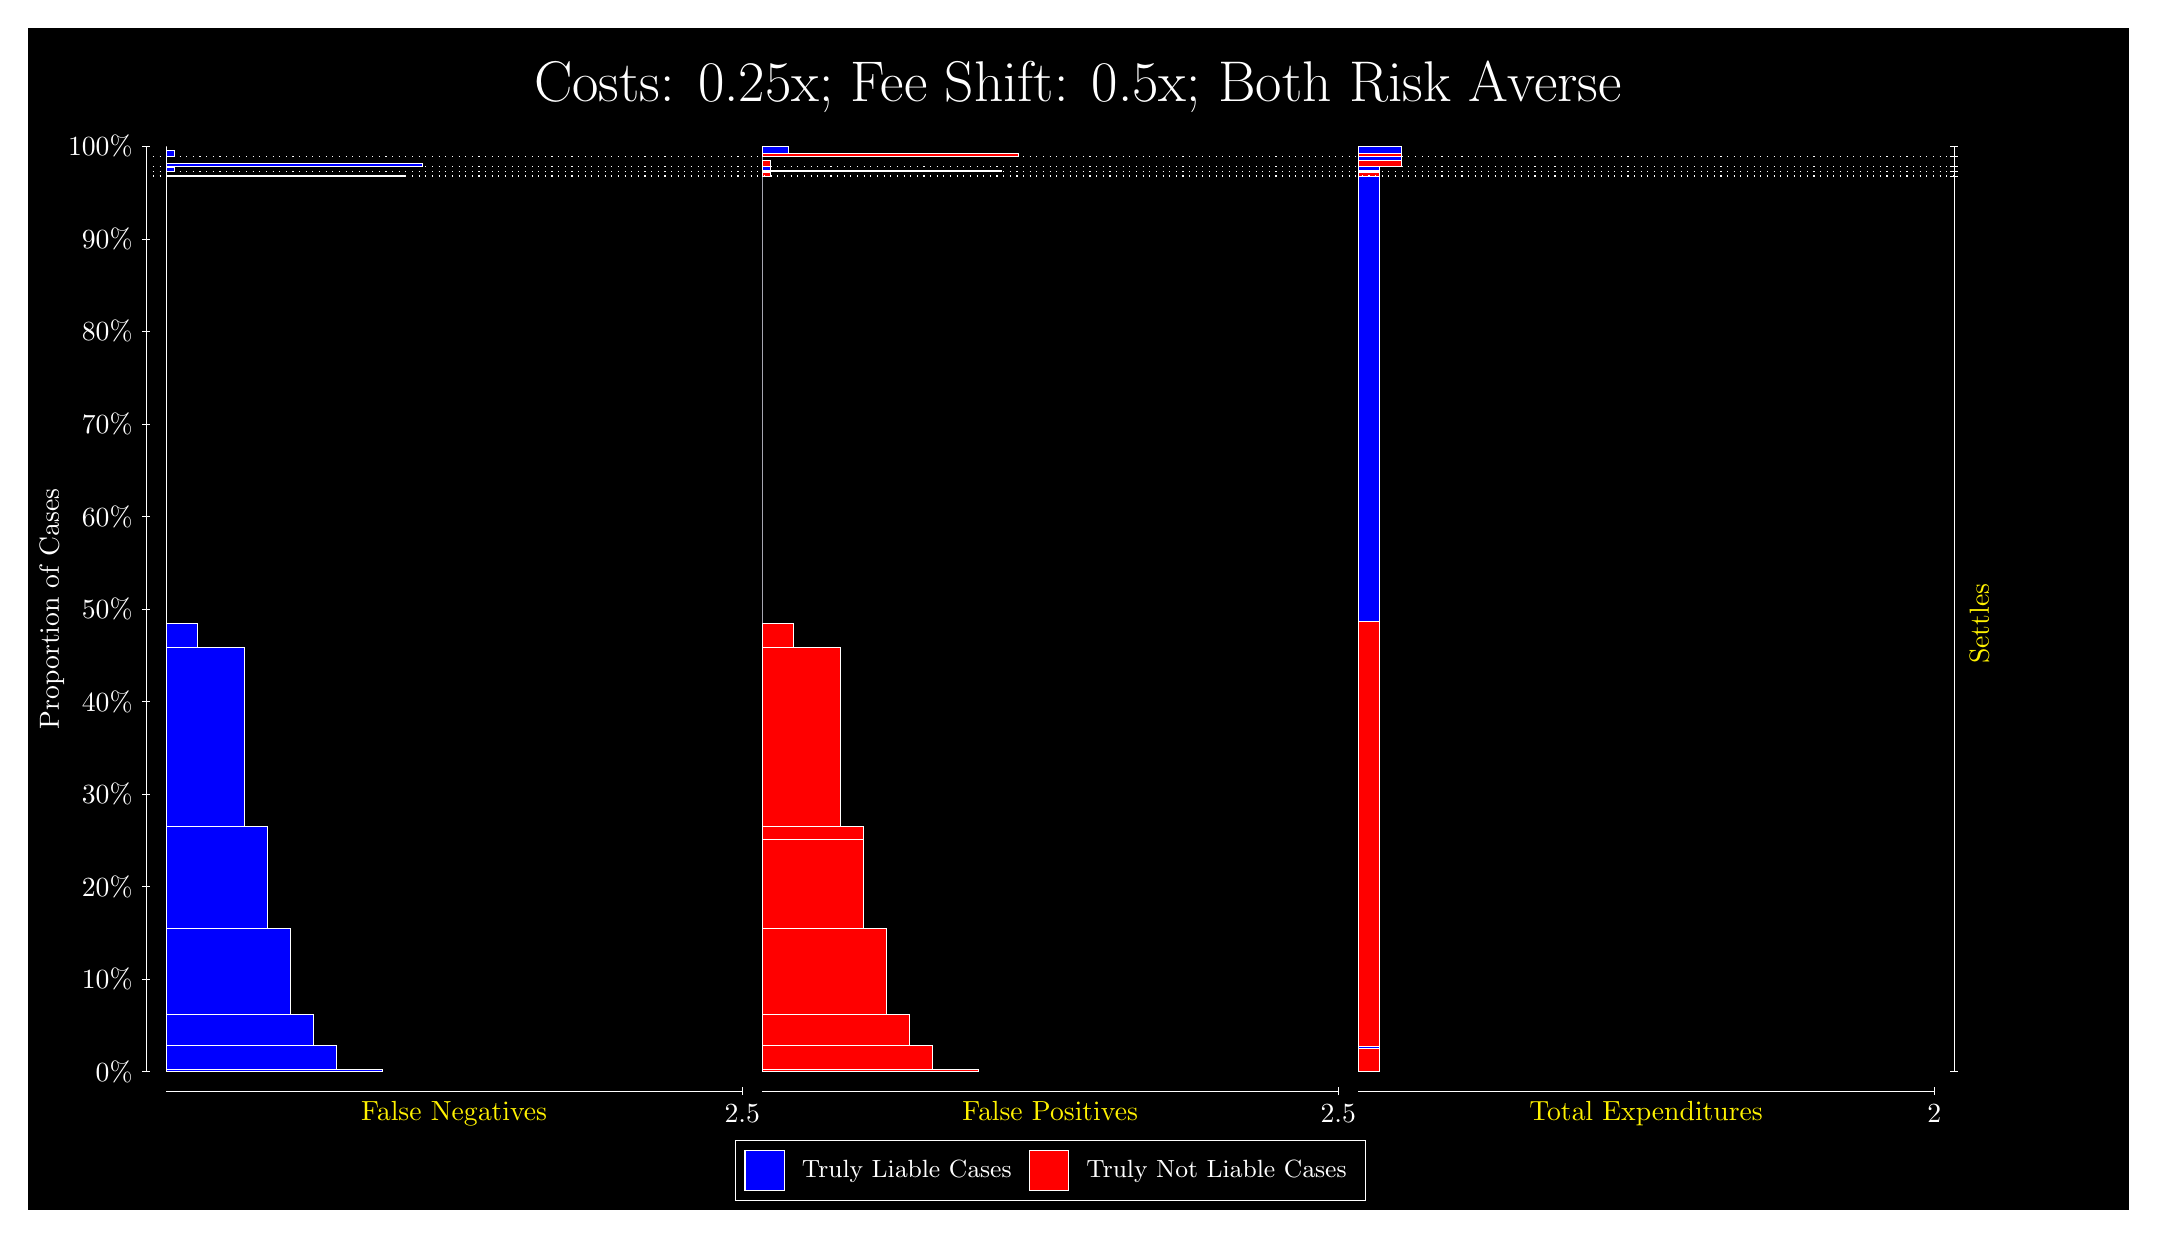
\begin{tikzpicture}
\draw[fill=black] (0,0) rectangle (26.667,15);
\draw[text=white] (0,13.5) rectangle (26.667,15) node[midway] {\huge Costs: 0.25x; Fee Shift: 0.5x; Both Risk Averse};
\draw[white, very thin] (1.5,1.75) -- (1.5,13.5);
\node[rotate=90, text=white, anchor=center] at (0.3, 7.625) {Proportion of Cases};
\draw[white, very thin] (1.45,1.75) -- (1.55,1.75);
\node[text=white, anchor=east] at (1.45, 1.75) {0\%};
\draw[white, very thin] (1.45,2.925) -- (1.55,2.925);
\node[text=white, anchor=east] at (1.45, 2.925) {10\%};
\draw[white, very thin] (1.45,4.1) -- (1.55,4.1);
\node[text=white, anchor=east] at (1.45, 4.1) {20\%};
\draw[white, very thin] (1.45,5.275) -- (1.55,5.275);
\node[text=white, anchor=east] at (1.45, 5.275) {30\%};
\draw[white, very thin] (1.45,6.45) -- (1.55,6.45);
\node[text=white, anchor=east] at (1.45, 6.45) {40\%};
\draw[white, very thin] (1.45,7.625) -- (1.55,7.625);
\node[text=white, anchor=east] at (1.45, 7.625) {50\%};
\draw[white, very thin] (1.45,8.8) -- (1.55,8.8);
\node[text=white, anchor=east] at (1.45, 8.8) {60\%};
\draw[white, very thin] (1.45,9.975) -- (1.55,9.975);
\node[text=white, anchor=east] at (1.45, 9.975) {70\%};
\draw[white, very thin] (1.45,11.15) -- (1.55,11.15);
\node[text=white, anchor=east] at (1.45, 11.15) {80\%};
\draw[white, very thin] (1.45,12.325) -- (1.55,12.325);
\node[text=white, anchor=east] at (1.45, 12.325) {90\%};
\draw[white, very thin] (1.45,13.5) -- (1.55,13.5);
\node[text=white, anchor=east] at (1.45, 13.5) {100\%};

\draw[white, very thin] (24.457,1.75) -- (24.457,13.5);
\draw[white, very thin] (24.407,1.75) -- (24.507,1.75);
\node[anchor=west] at (24.407, 1.75) {};
\draw[white, very thin] (24.407,13.123) -- (24.507,13.123);
\node[anchor=west] at (24.407, 13.123) {};
\draw[white, very thin] (24.407,13.183) -- (24.507,13.183);
\node[anchor=west] at (24.407, 13.183) {};
\draw[white, very thin] (24.407,13.243) -- (24.507,13.243);
\node[anchor=west] at (24.407, 13.243) {};
\draw[white, very thin] (24.407,13.372) -- (24.507,13.372);
\node[anchor=west] at (24.407, 13.372) {};
\draw[white, very thin] (24.407,13.5) -- (24.507,13.5);
\node[anchor=west] at (24.407, 13.5) {};

\draw[white, very thin, fill=blue] (1.75,1.75) rectangle (4.4946,1.7751);
\draw[white, very thin, fill=blue] (1.75,1.7751) rectangle (3.9091,2.0813);
\draw[white, very thin, fill=blue] (1.75,2.0813) rectangle (3.6163,2.4747);
\draw[white, very thin, fill=blue] (1.75,2.4747) rectangle (3.3236,3.5654);
\draw[white, very thin, fill=blue] (1.75,3.5654) rectangle (3.0308,4.8624);
\draw[white, very thin, fill=blue] (1.75,4.8624) rectangle (2.738,7.1426);
\draw[white, very thin, fill=blue] (1.75,7.1426) rectangle (2.1525,7.4366);
\draw[white, very thin, fill=red] (1.75,7.4366) rectangle (1.75,13.123);
\draw[white, very thin, fill=blue] (1.75,13.123) rectangle (4.7873,13.134);
\draw[white, very thin, fill=red] (1.75,13.134) rectangle (1.75,13.183);
\draw[white, very thin, fill=blue] (1.75,13.183) rectangle (1.8598,13.233);
\draw[white, very thin, fill=red] (1.75,13.233) rectangle (1.75,13.243);
\draw[white, very thin, fill=blue] (1.75,13.243) rectangle (5.0069,13.287);
\draw[white, very thin, fill=red] (1.75,13.287) rectangle (1.75,13.372);
\draw[white, very thin, fill=blue] (1.75,13.372) rectangle (1.8598,13.456);
\draw[white, very thin, fill=red] (1.75,13.456) rectangle (1.75,13.5);
\draw[white, very thin, fill=red] (9.3189,1.75) rectangle (12.063,1.7751);
\draw[white, very thin, fill=red] (9.3189,1.7751) rectangle (11.478,2.0813);
\draw[white, very thin, fill=red] (9.3189,2.0813) rectangle (11.185,2.4747);
\draw[white, very thin, fill=red] (9.3189,2.4747) rectangle (10.892,3.5654);
\draw[white, very thin, fill=red] (9.3189,3.5654) rectangle (10.6,4.7045);
\draw[white, very thin, fill=red] (9.3189,4.7045) rectangle (10.6,4.8624);
\draw[white, very thin, fill=red] (9.3189,4.8624) rectangle (10.307,7.1427);
\draw[white, very thin, fill=red] (9.3189,7.1427) rectangle (9.7214,7.4367);
\draw[white, very thin, fill=blue] (9.3189,7.4367) rectangle (9.3189,13.123);
\draw[white, very thin, fill=red] (9.3189,13.123) rectangle (9.4287,13.173);
\draw[white, very thin, fill=blue] (9.3189,13.173) rectangle (9.3189,13.183);
\draw[white, very thin, fill=red] (9.3189,13.183) rectangle (12.356,13.194);
\draw[white, very thin, fill=blue] (9.3189,13.194) rectangle (9.4287,13.243);
\draw[white, very thin, fill=red] (9.3189,13.243) rectangle (9.4287,13.328);
\draw[white, very thin, fill=blue] (9.3189,13.328) rectangle (9.3189,13.372);
\draw[white, very thin, fill=red] (9.3189,13.372) rectangle (12.576,13.415);
\draw[white, very thin, fill=blue] (9.3189,13.415) rectangle (9.6482,13.5);
\draw[white, very thin, fill=red] (16.888,1.75) rectangle (17.162,2.0439);
\draw[white, very thin, fill=blue] (16.888,2.0439) rectangle (17.162,2.0691);
\draw[white, very thin, fill=red] (16.888,2.0691) rectangle (17.162,7.4618);
\draw[white, very thin, fill=blue] (16.888,7.4618) rectangle (17.162,13.123);
\draw[white, very thin, fill=red] (16.888,13.123) rectangle (17.162,13.173);
\draw[white, very thin, fill=blue] (16.888,13.173) rectangle (17.162,13.183);
\draw[white, very thin, fill=red] (16.888,13.183) rectangle (17.162,13.194);
\draw[white, very thin, fill=blue] (16.888,13.194) rectangle (17.162,13.243);
\draw[white, very thin, fill=red] (16.888,13.243) rectangle (17.437,13.328);
\draw[white, very thin, fill=blue] (16.888,13.328) rectangle (17.437,13.372);
\draw[white, very thin, fill=red] (16.888,13.372) rectangle (17.437,13.415);
\draw[white, very thin, fill=blue] (16.888,13.415) rectangle (17.437,13.5);
\draw[white, dotted] (1.5,13.123) -- (24.457,13.123);
\draw[white, dotted] (1.5,13.183) -- (24.457,13.183);
\draw[white, dotted] (1.5,13.243) -- (24.457,13.243);
\draw[white, dotted] (1.5,13.372) -- (24.457,13.372);
\draw[white, very thin] (1.75,1.5) -- (9.0689,1.5);
\node[text=yellow, anchor=north] at (5.4094, 1.5) {False Negatives};
\draw[white, very thin] (9.0689,1.45) -- (9.0689,1.55);
\node[text=white, anchor=north] at (9.0689, 1.45) {2.5};

\draw[white, very thin] (9.3189,1.5) -- (16.638,1.5);
\node[text=yellow, anchor=north] at (12.978, 1.5) {False Positives};
\draw[white, very thin] (16.638,1.45) -- (16.638,1.55);
\node[text=white, anchor=north] at (16.638, 1.45) {2.5};

\draw[white, very thin] (16.888,1.5) -- (24.207,1.5);
\node[text=yellow, anchor=north] at (20.547, 1.5) {Total Expenditures};
\draw[white, very thin] (24.207,1.45) -- (24.207,1.55);
\node[text=white, anchor=north] at (24.207, 1.45) {2};

\node[text=yellow, centered, rotate=90] at (24.777, 7.4366) {Settles};





\draw (12.978300999999998,1.5) node[draw=none] (baseCoordinate) {};
\begin{scope}[align=center]
        \matrix[scale=0.5, draw=white, below=0.5cm of baseCoordinate, nodes={draw}, column sep=0.1cm]{
            \node[rectangle, draw, minimum width=0.5cm, minimum height=0.5cm, fill=blue] {}; &
            \node[draw=none, font=\small, text=white] (B) {Truly Liable Cases}; &
            \node[rectangle, draw, minimum width=0.5cm, minimum height=0.5cm, fill=red] {}; &
            \node[draw=none, font=\small, text=white] (B) {Truly Not Liable Cases}; \\
            };
\end{scope}

\end{tikzpicture}
\end{document}